%======================================================%
%   Beamer Presentation
%   LaTeX Template
%   compile using PDFTeXify or PDFLaTeX
%======================================================%

\documentclass[notheorems,11pt,compress]{beamer}

\mode<presentation>{
\usetheme{Madrid}
\usecolortheme{rose}
\usefonttheme[onlymath]{serif}
\setbeamertemplate{blocks}[rounded][shadow=true]
\setbeamertemplate{navigation symbols}{}
}

\usepackage[english]{babel}
\usepackage{amsmath,amssymb,version}
\usepackage{graphicx,fancybox,mathrsfs,multirow}
\usepackage{booktabs}
\usepackage{epsfig,epstopdf}
\usepackage{url,hyperref}
\usepackage{tabularx,array,makecell}
\usepackage{color,xcolor}
\usepackage{cases}
\usepackage{mathtools}
\usepackage{tikz}

\definecolor{utaBluePrimary}{HTML}{0064B1}
\definecolor{lightgray}{RGB}{240, 240, 240}
\definecolor{lightorange}{HTML}{F58025}

\newcommand{\utaBlue}[1]{\textcolor{utaBluePrimary}{#1}}

\setbeamercolor*{palette primary}{bg=utaBluePrimary}
\setbeamercolor*{palette secondary}{bg=utaBluePrimary, fg=white}
\setbeamercolor*{palette tertiary}{bg=utaBluePrimary, fg=white}
\setbeamercolor*{titlelike}{bg=utaBluePrimary, fg=white}
\setbeamercolor*{title}{bg=utaBluePrimary, fg=white}
\setbeamercolor*{caption name}{fg=utaBluePrimary}
\setbeamercolor*{page number in head/foot}{bg=utaBluePrimary, fg=white}
\setbeamercolor*{date in head/foot}{bg=utaBluePrimary,fg=white}
\setbeamercolor*{section in toc}{fg=utaBluePrimary}
\setbeamercolor*{section number projected}{fg=white, bg=utaBluePrimary}
\setbeamercolor*{subsection number projected}{fg=white, bg=utaBluePrimary}
\setbeamercolor*{item}{fg=black}

\AtBeginSection[]{
\begin{frame}
  \frametitle{Outline}
  \tableofcontents[currentsection,currentsubsection,subsectionstyle=show/show/shaded]
  \addtocounter{framenumber}{-1}
\end{frame}
}

\graphicspath{{./figs/}{./logos/}{./}} % Add all relevant image directories

\title[USDA Summer Intern Meeting]{USDA Summer Intern Meeting: Opening Presentation}
\author{Jose Andres Cortes}
\institute[UTA]{
Department of Mathematics \\
University of Texas at Arlington \\
\medskip
\textit{In collaboration with: Dr. Korzeniowski, Dr. Tolbert, Dr. Galina, Dr. Kravetski (USDA-ARS)}
}
\date[May 27, 2025]{May 27, 2025}
\titlegraphic{
\includegraphics[width=2.5cm]{utaLogo.png}} % Remove 'logos/' since it's in \graphicspath, and use .jpg

\begin{document}

\setlength{\baselineskip}{15pt}

%------------------- Title Slide -------------------
\begin{frame}
\titlepage
\end{frame}

%------------------- Outline -------------------
\begin{frame}
\frametitle{Outline}
\tableofcontents[hideallsubsections]
\end{frame}

%------------------- Introduction -------------------
% \section{Introduction}

% \begin{frame}
% \frametitle{Welcome}
% \begin{block}{}
% \textbf{Good Morning everyone!\ } My name is Jose Andres Cortes. This will be my third summer with the USDA. I am currently a PhD student at the Department of Mathematics, University of Texas at Arlington, funded as a GRA by the USDA.
% \end{block}
% \end{frame}

% %------------------- Meet the Team -------------------
\section{Meet the Team}

\begin{frame}
\frametitle{Meet the Team}
\begin{columns}
\column{0.55\textwidth}
\begin{itemize}
    \item Dr.\@ Korzeniowski (UTA)
    \item Dr.\@ Tolbert (USDA-ARS)
    \item Dr.\@ Galina (USDA-ARS)
    \item Dr.\@ Kravetski (USDA-ARS)
\end{itemize}
\vspace{1em}
\small
\textit{We are working on the MINS project, using gamma spectroscopy to measure soil carbon content in the field.\ }
% \column{0.45\textwidth}
% \includegraphics[width=\linewidth]{team_photo.jpg}
\end{columns}
\end{frame}

\begin{frame}
\frametitle{The MINS Project}
\begin{columns}
\column{0.5\textwidth}
\includegraphics[width=\linewidth]{machine.png}
\column{0.5\textwidth}
\includegraphics[width=\linewidth]{meandmachine.png}
\end{columns}
\vspace{1em}
\small
\textit{This is the machine we're working on. This is me next to the machine during my visit to the lab in Auburn, Alabama. The machine is called \textbf{MINS} (Mobile In Situ Spectroscopy).}
\end{frame}

%------------------- Development -------------------
\section{Project Development}

\begin{frame}
\frametitle{Project Development}
\begin{itemize}
    \item USDA develops and tests the physical MINS machine.
    \item \textbf{My role:} Mathematical and statistical support.
    \item Two main focus areas:
    \begin{itemize}
        \item Simulation
        \item Data Analysis
    \end{itemize}
\end{itemize}
\end{frame}

%------------------- Simulation -------------------
\section{Simulation}

\begin{frame}
\frametitle{Simulation}
\begin{columns}
\column{0.5\textwidth}
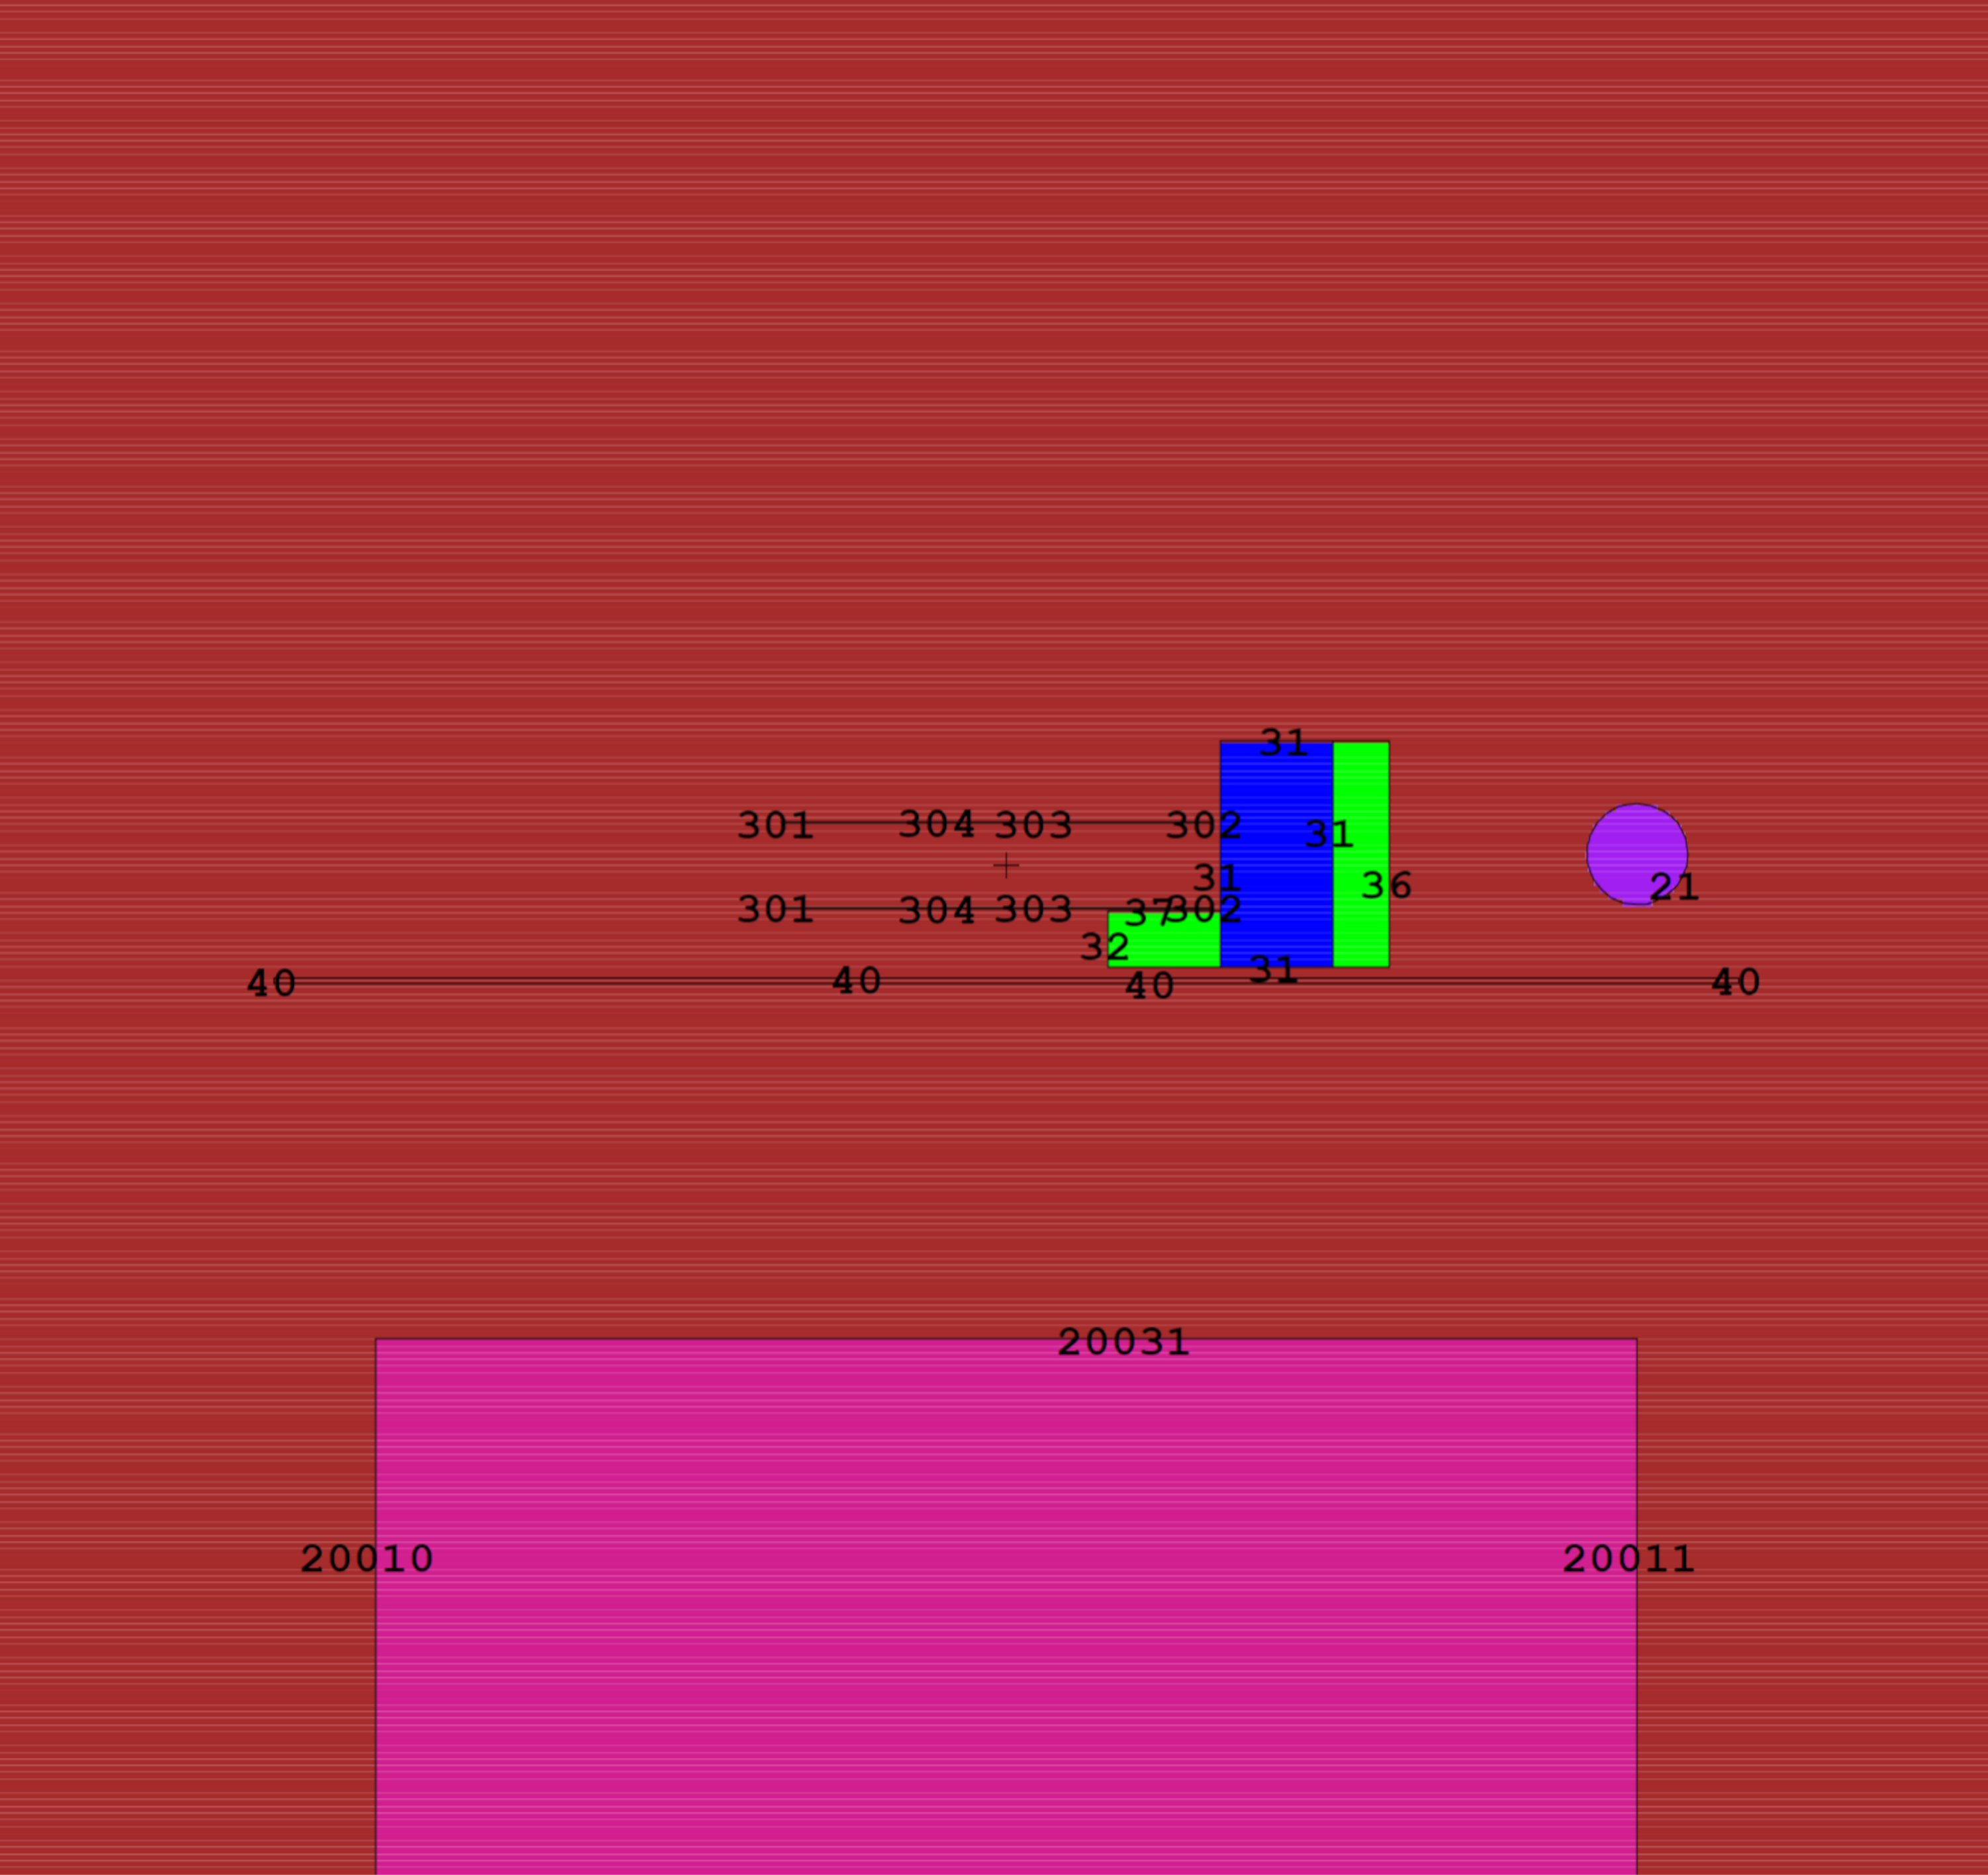
\includegraphics[width=\linewidth]{minsinmcnp.png}
\column{0.5\textwidth}
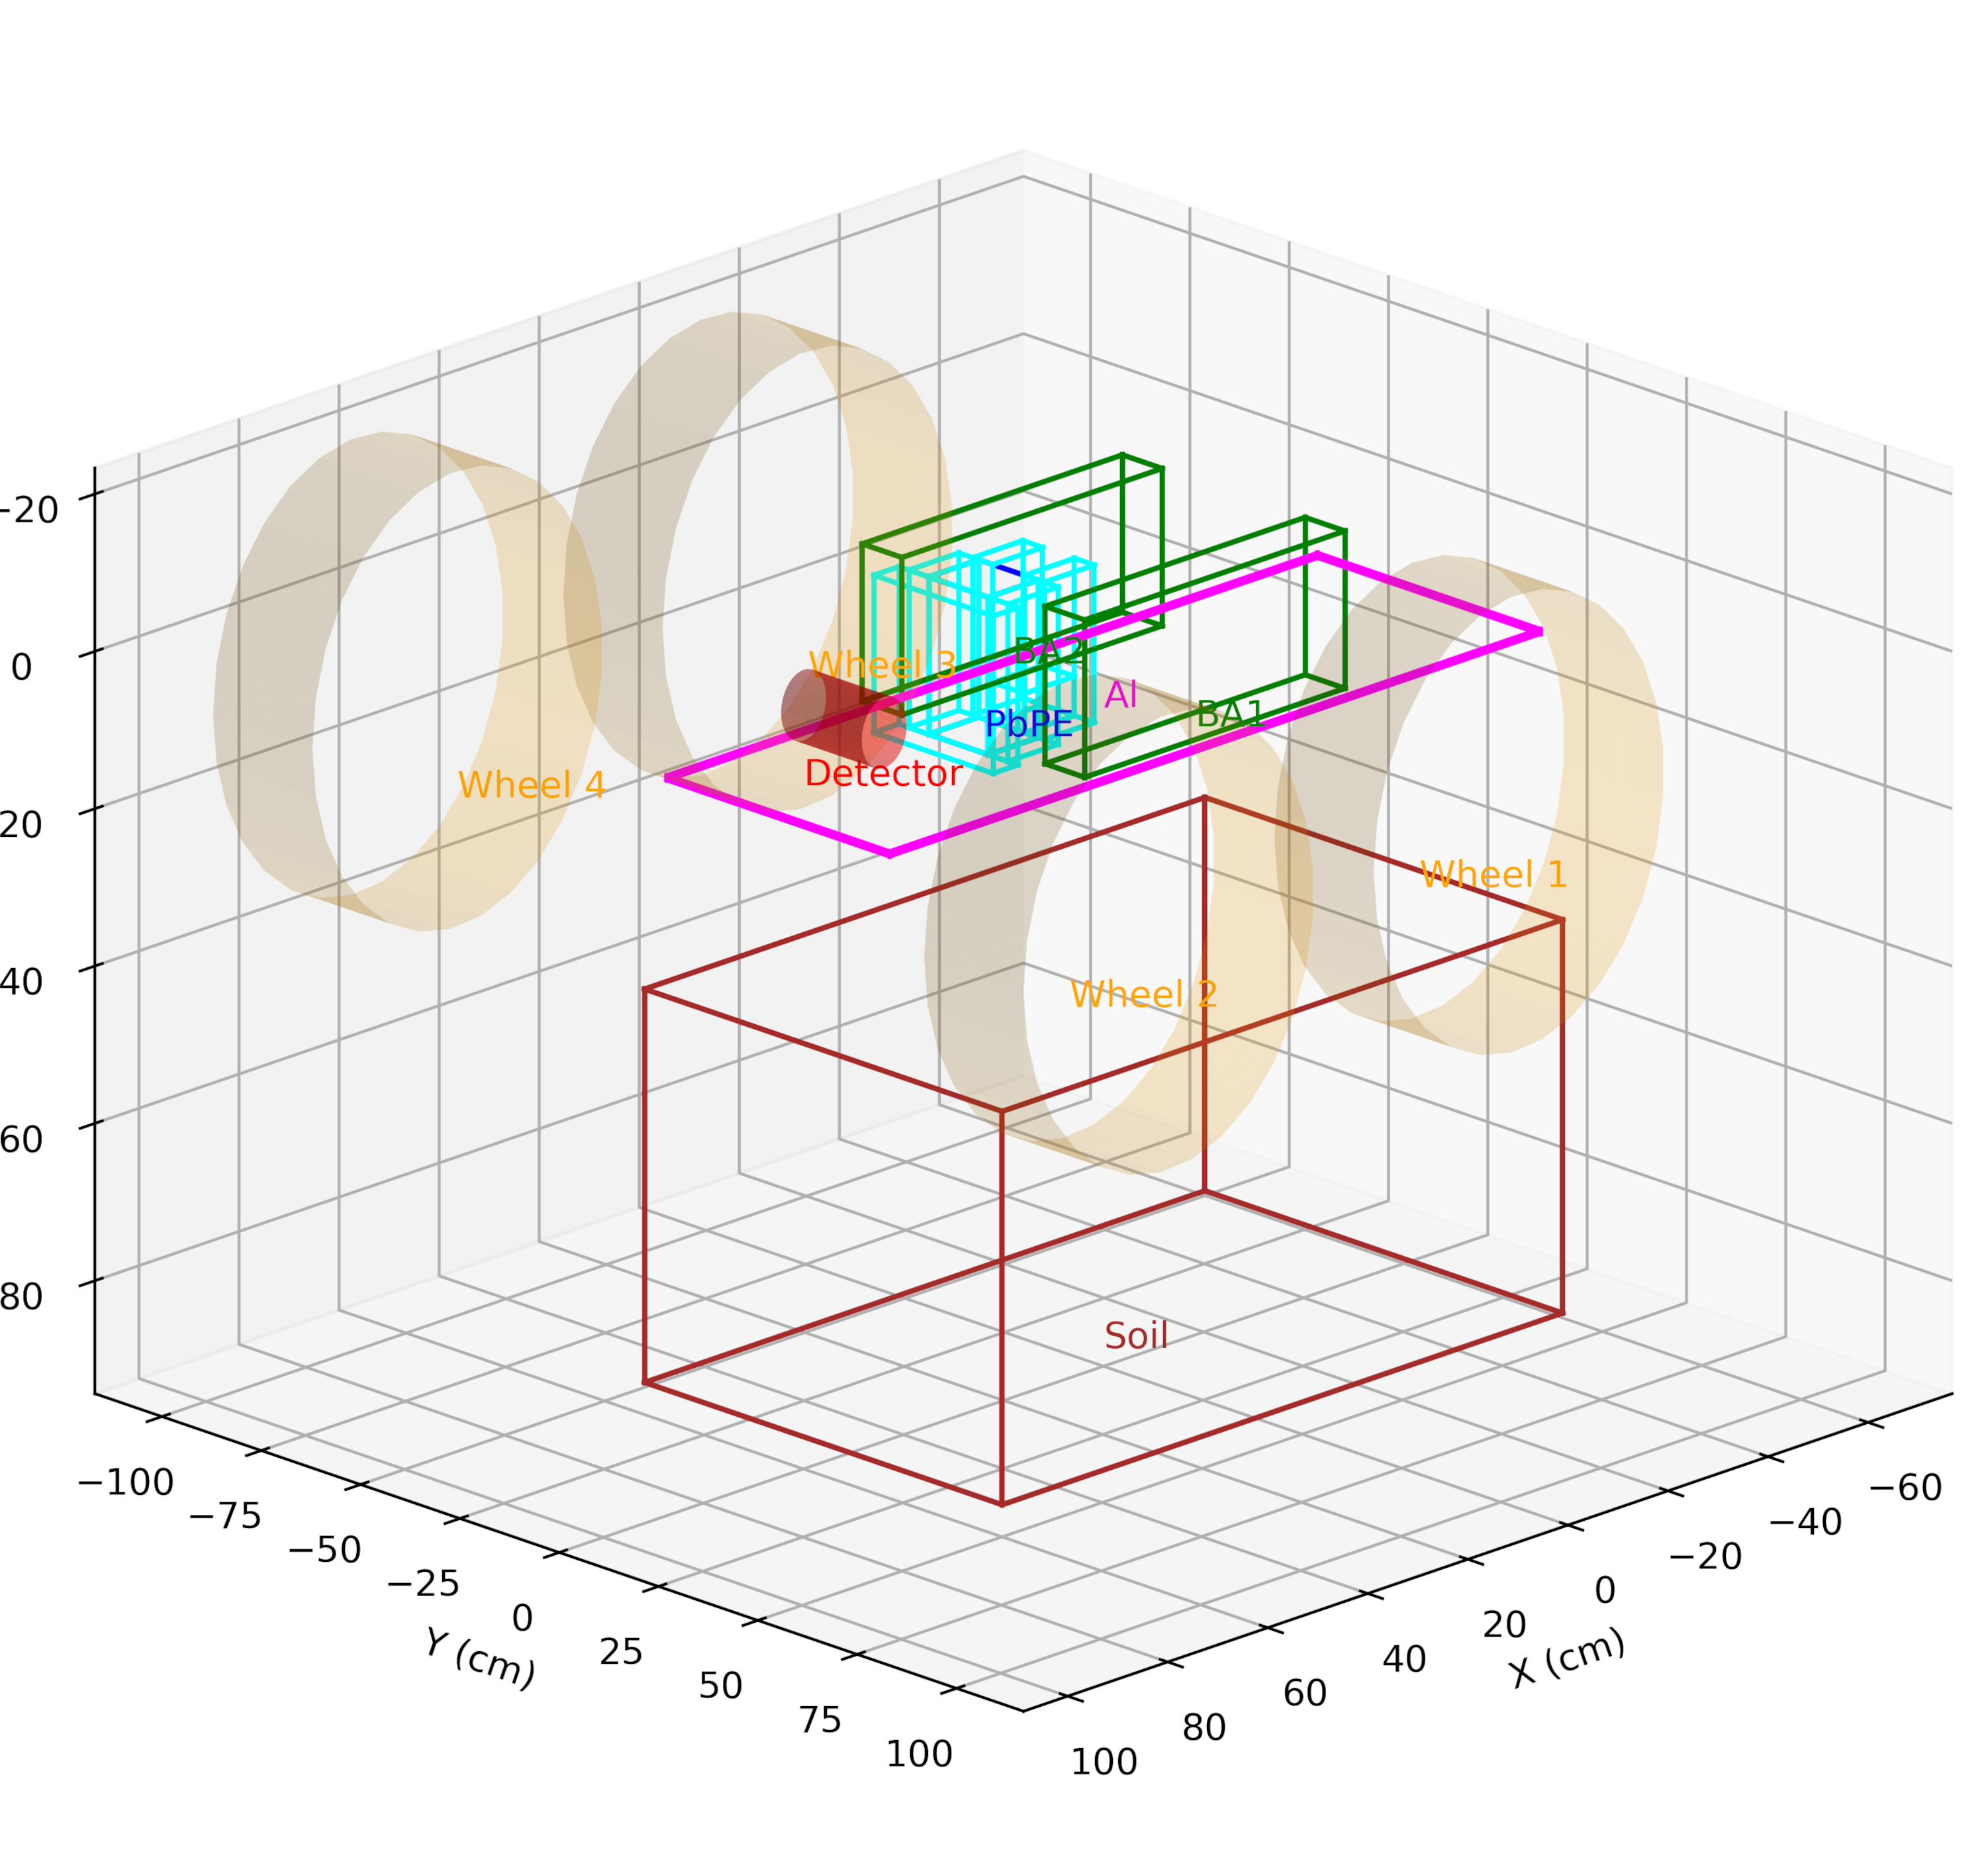
\includegraphics[width=\linewidth]{minsin3d.png}
\end{columns}
\vspace{1em}
\begin{itemize}
    \item Simulate MINS using Monte Carlo particle methods (MCNP).
    \item Predict machine performance in various scenarios.
\end{itemize}
\small
\textit{We use the national code MCNP to simulate the MINS results and predict the performance of the machine in different scenarios.}
\end{frame}

\begin{frame}
\frametitle{Recent Work in Simulation}
\begin{center}
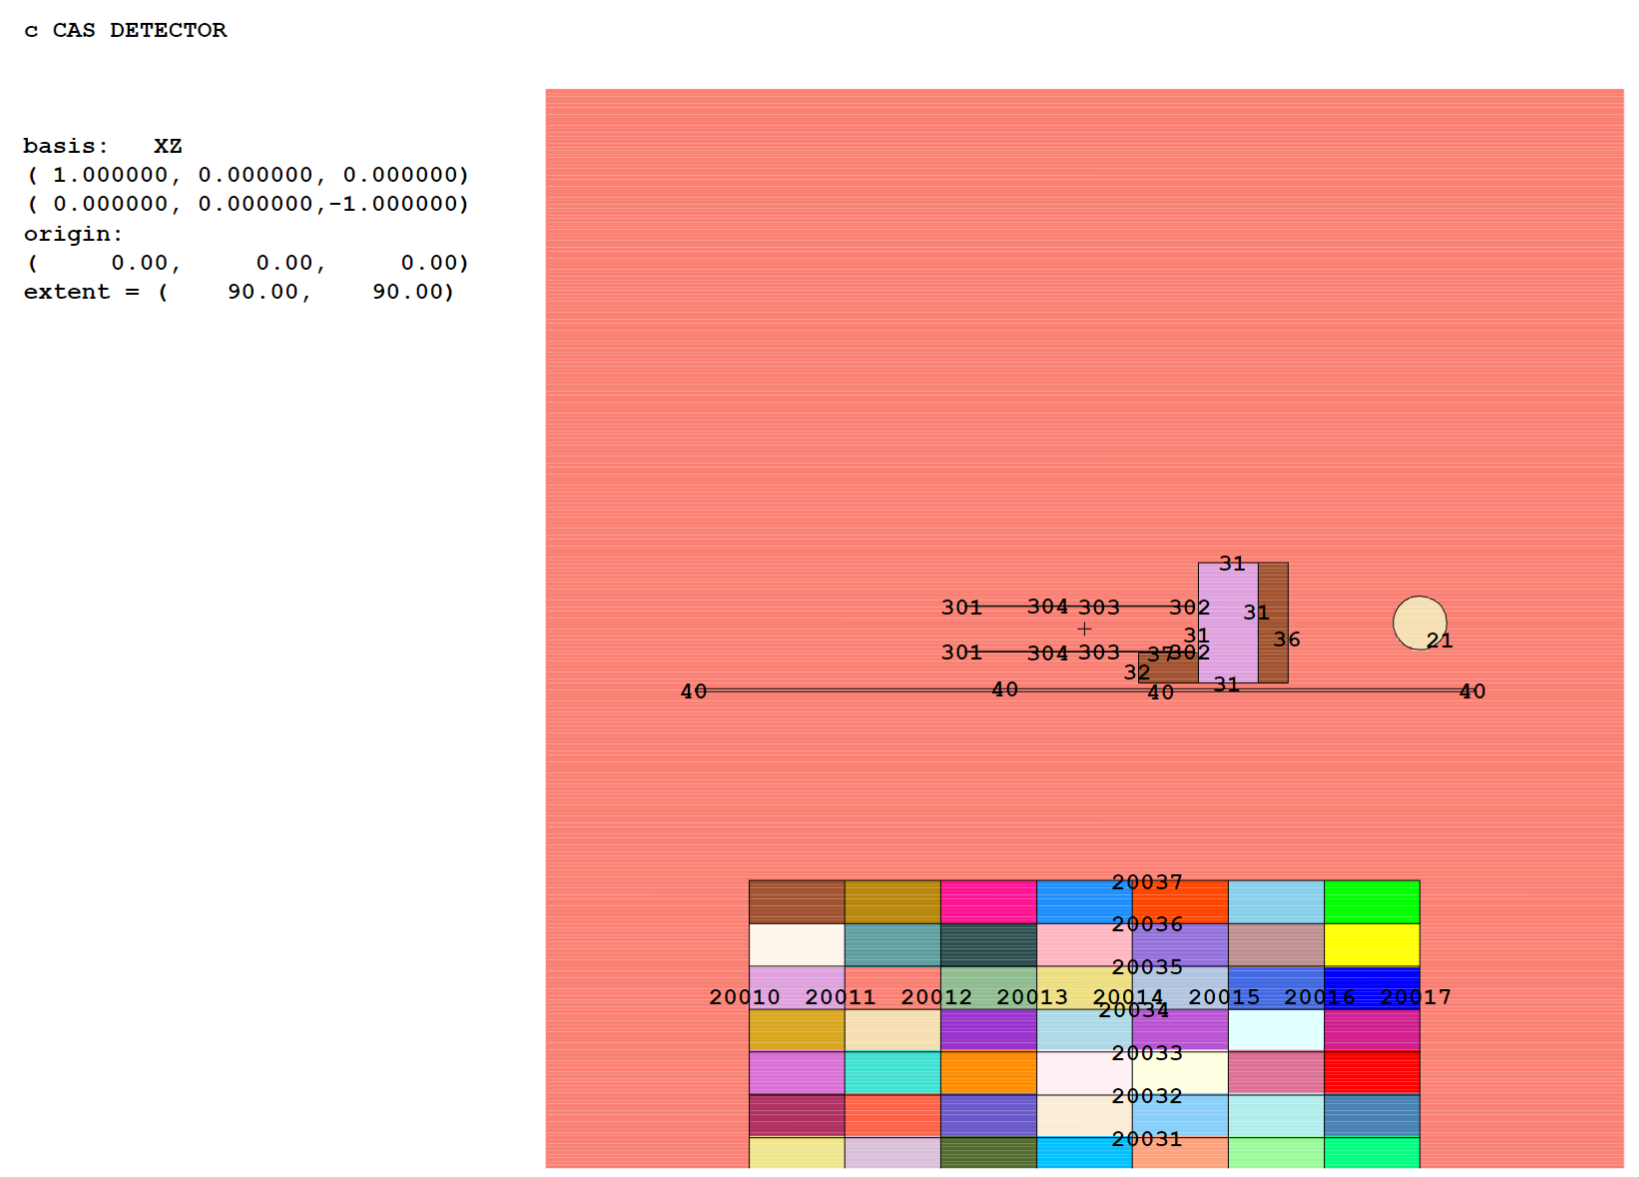
\includegraphics[width=0.7\linewidth]{7x7x7inmcnp.png}
\end{center}
\small
\textit{Recent work: Introduced functionalized soil samples. Previously, samples were simulated as chemically even; now, we simulate them as digitized functions of spatial dimensions for more realistic data.}
\end{frame}

%------------------- Data Analysis -------------------
\section{Data Analysis}

\begin{frame}
\frametitle{Analysis}
\begin{center}
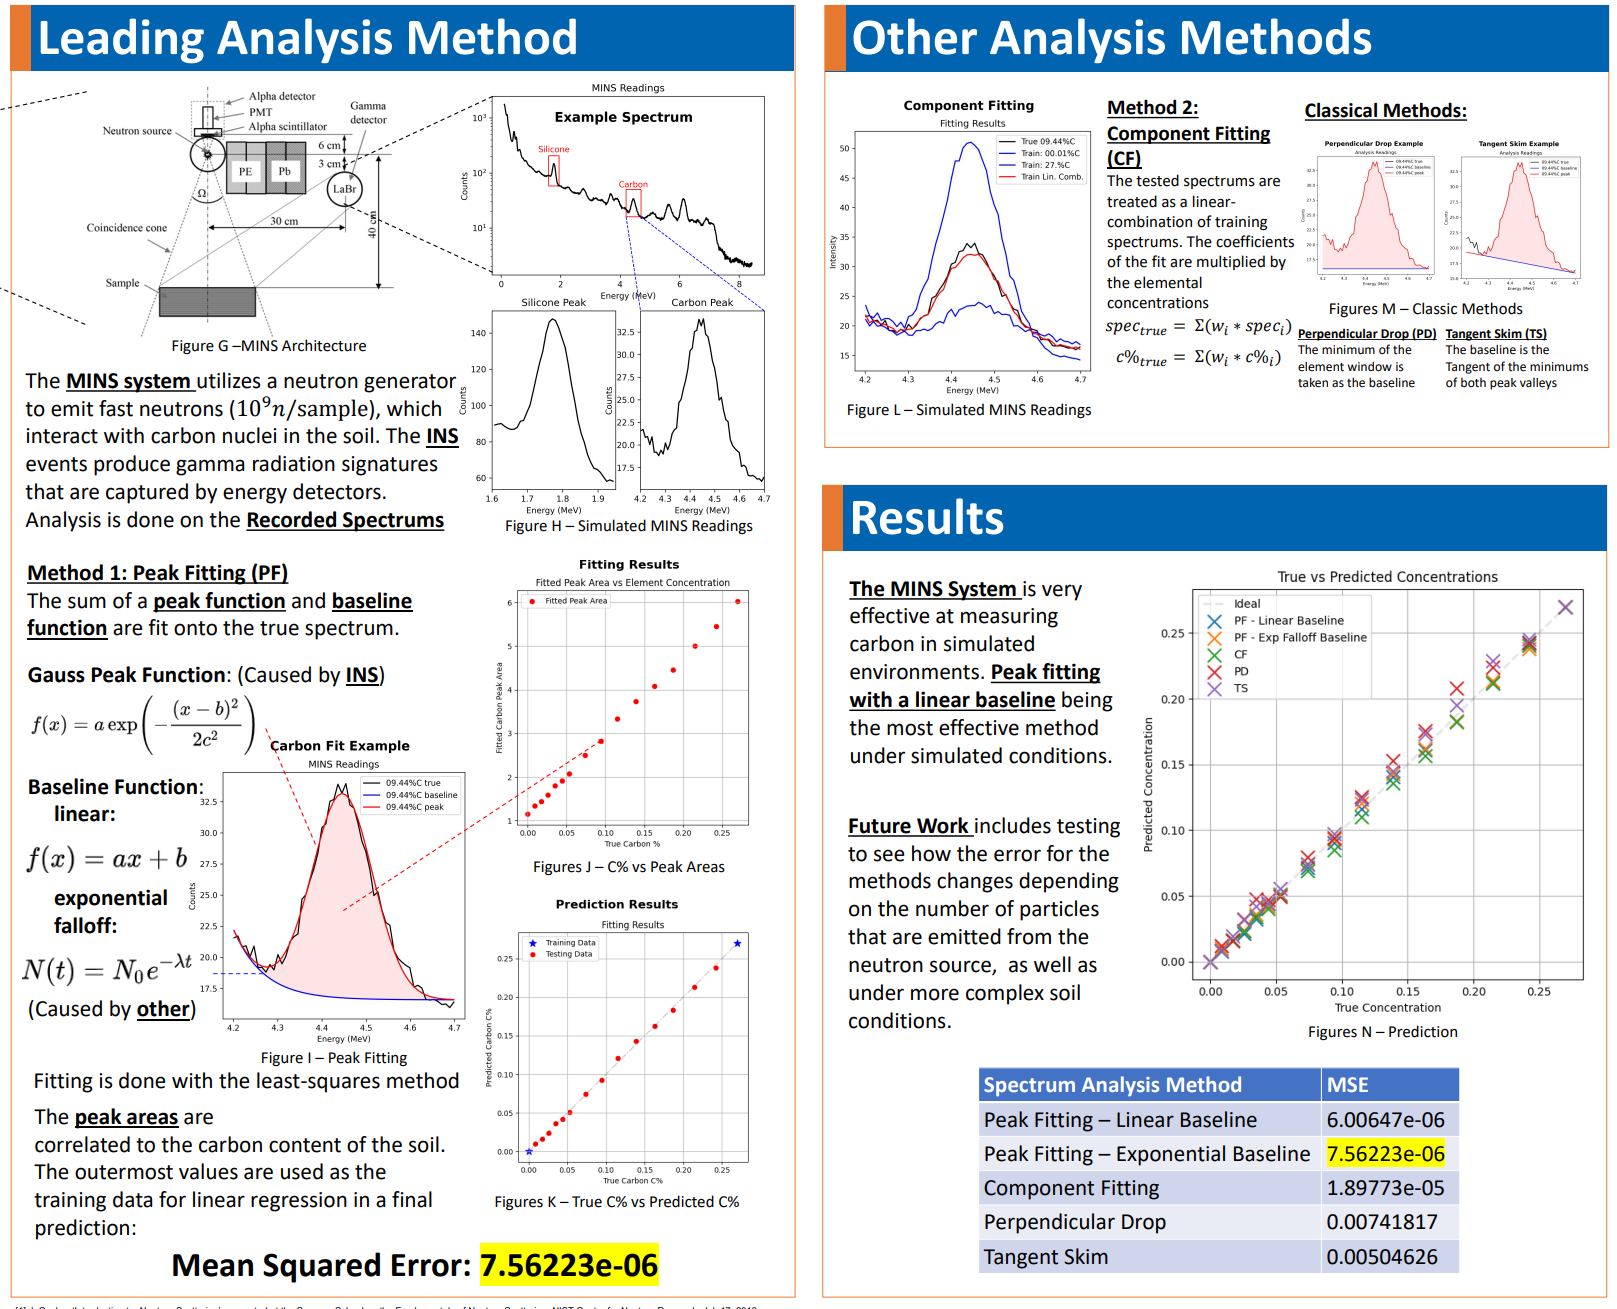
\includegraphics[width=0.7\linewidth]{analysismethods.png}
\end{center}
\small
\textit{Second area: Analysis of the data obtained from MINS. Last year, I focused on analysis methods for the spectrum recorded by the machine.}
\end{frame}

%------------------- Goals -------------------
\section{Goals and Steps}

\begin{frame}
\frametitle{Goals for This Summer}
\begin{enumerate}
    \item Develop and evaluate mathematical methods for new machine architecture.
    \item Detection Range (Depth) study of the MINS machine.
    \item Comparison of MINS and soil core measurements.
    \item Mapping the results of the machine onto a field.
    \item Estimation of the impact of the surface area sampled on field measurements.
\end{enumerate}
\small
\textit{Overall, these goals are about mathematically testing the capability of the machine.}
\end{frame}

\begin{frame}
\frametitle{Project Steps}
\begin{enumerate}
    \item Generate Pure Spectrums (Spectrum Generation)
    \item Generate Effective Map (Associative Map)
    \item Try Fast Spectrum Convolution (Spectrum Generation)
    \item Compare Analysis Methods (Apply previous code to new data)
    \item Variance Study
    \item Depth Study
    \item Core Harvesting Comparison (local)
    \item Mapping Comparison
    \item Field Coverage Study
\end{enumerate}
\end{frame}

\begin{frame}
\frametitle{First Steps Completed}
\begin{center}
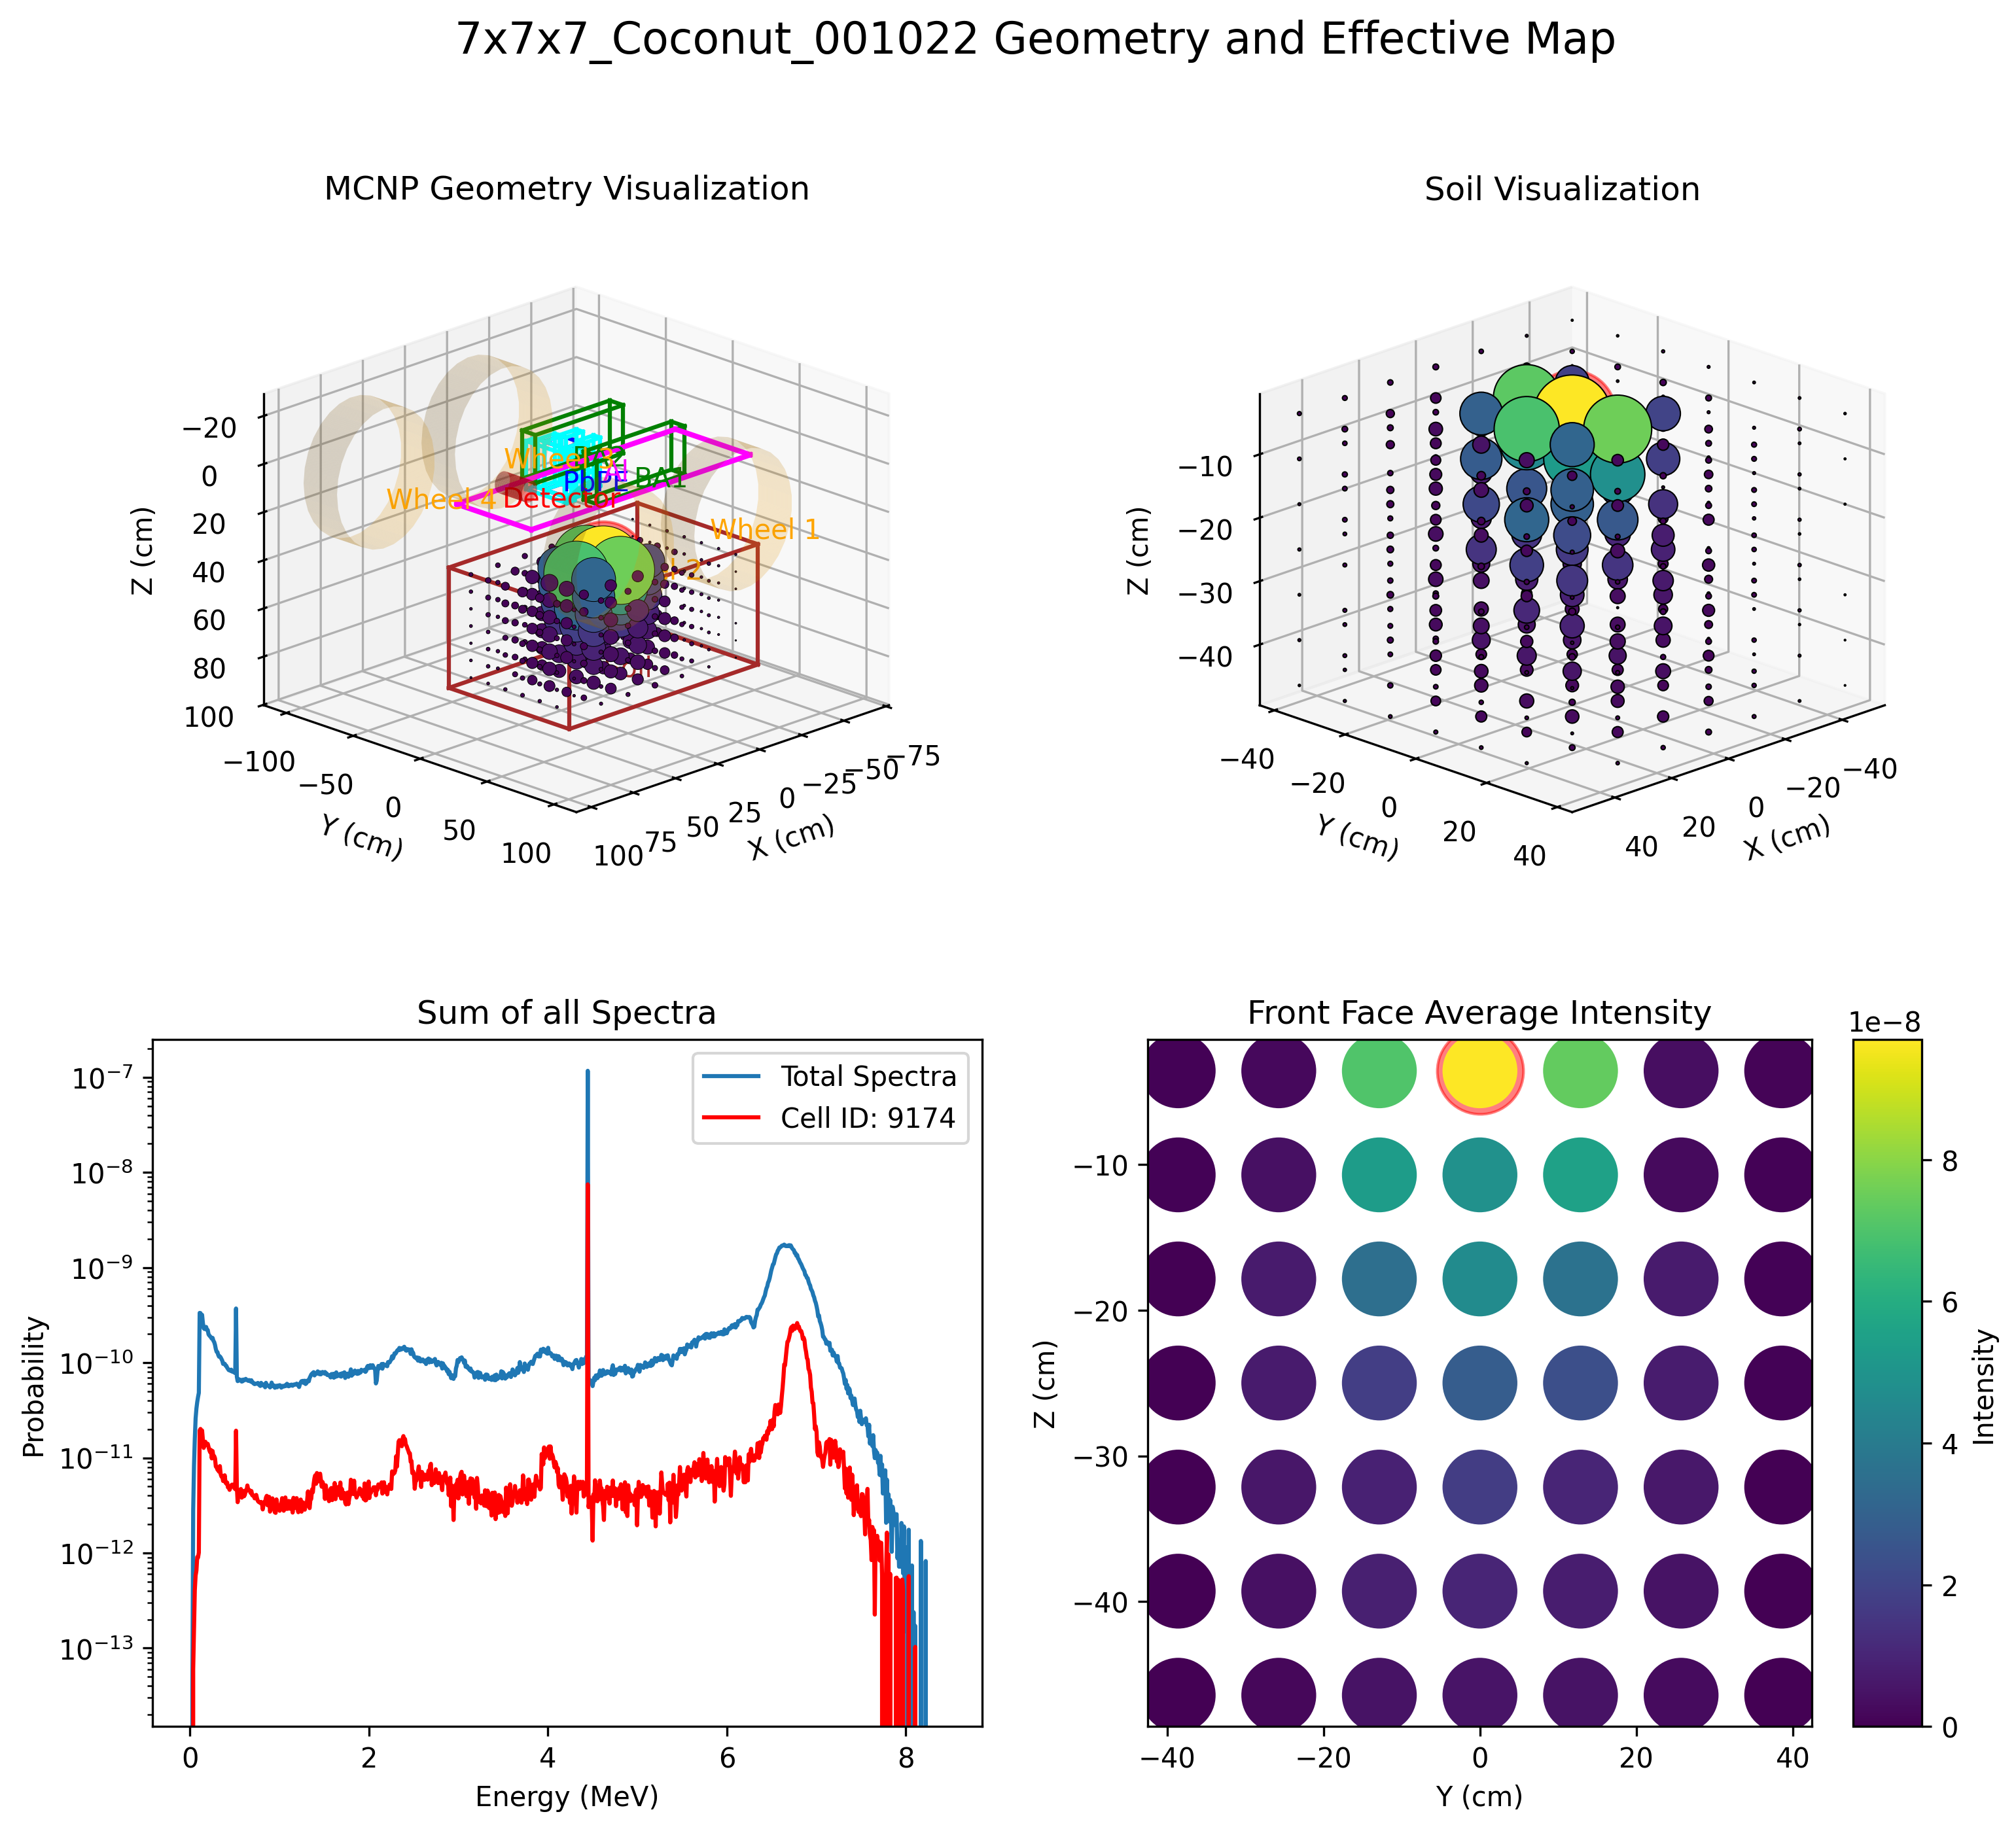
\includegraphics[width=0.7\linewidth]{detectorrange.png}
\end{center}
\small
\textit{First and second steps completed: data augmentation, including a map of how the sample is scanned. This achieves the goal of measuring range in simulation.}
\end{frame}

%------------------- End Slide -------------------
\section*{Questions}

\begin{frame}
\frametitle{Questions?}
\begin{center}
\LARGE{Any questions, comments, concerns?}\\[2em]
\Huge{\textcolor[RGB]{255,0,0}{Thank you!}}
\end{center}
\end{frame}

\end{document}